% x

% \usepackage{pgfplots}
% \usetikzlibrary{calc}
% \usepgfplotslibrary{colormaps}


\RequirePackage[l2tabu, orthodox]{nag}
\documentclass[12pt]{article}
\usepackage{geometry}                % See geometry.pdf to learn the layout options. There are lots.
\geometry{letterpaper}
\usepackage[autostyle=false, style=english]{csquotes}
\usepackage{mathtools}
%\MakeOuterQuote{"}
\setlength{\marginparwidth}{2cm}

\usepackage{nomencl}
\makenomenclature
% Run the following command in terminal to update:
% makeindex "main.nlo" -s nomencl.ist -o "main.nls"
\nomenclature{$f, f_c$}{The map $z \mapsto z^2+c.$}
\nomenclature{$\mathcal J$}{The Julia set of $f$.}
\nomenclature{$K$}{The filled Julia set of $f$.}
\nomenclature{$\gamma_{z_1, z_2}$}{The track connecting $z_1$ and $z_2$. It can be either angular (\enquote{peripheral}) or radial (\enquote{express}).}
\nomenclature{$\eta_{z_1, z_2}$}{The itinerary connecting two points. When $z_1$ and $z_2$ are stations, this is the same as $\gamma_{z_1,z_2}$.}
\nomenclature{$A_\infty(f_c)$}{The exterior of the Julia set of $f_c$. The complement of $K_c$.}
\nomenclature{$\mathrm{Exterior}(\mathcal{J})$}{ $\;$ An Alternative notation for $A_\infty(f_c)$.}
\nomenclature{$\psi$}{The Böttcher coordinate $\mathbb D ^* \to \Exterior(\mathcal J)$ conjugating $f_0$ and $f$.}
\nomenclature{$s_{n,k}$}{A station in $\mathbb D^*$ or its image under $\psi$.}
\nomenclature{$\Delta (\gamma, \mathcal P)$}{The relative distance to the post-critical set.}
\nomenclature{$I_{n}$}{The $n$-th departure set.}
\nomenclature{$\ell_n$ }{$\Length([s_{n},s_{n+1}]) = s_{n,0}-s_{n+1,0}.$}
\nomenclature{$\alpha_n$}{the union of the two outermost tracks emanating from the station $s_{n,0}$.}


% Prevents line breaks at math inline
\relpenalty=9999
\binoppenalty=9999

\usepackage{graphicx,color,mathtools}
\usepackage{amssymb,amsmath,amsthm,mathrsfs}
%\usepackage[all,cmtip]{xy}
\usepackage{comment}
%\usepackage{todonotes}
\usepackage{enumitem}   
\usepackage{tikz} 
\usepackage{pgfplots}
\pgfplotsset{compat=1.18}
\usepackage{graphicx}
\usepackage{xcolor}

\usepackage{hyperref}
\usepackage[capitalize,nameinlink,noabbrev]{cleveref}

\usepackage[pdftex,bookmarks,pdfnewwindow,plainpages=false,unicode,pdfencoding=auto]{}


\DeclareGraphicsRule{.tif}{png}{.png}{`convert #1 `dirname #1`/`basename #1 .tif`.png}
\linespread{1.2}

\numberwithin{equation}{section}

\newtheorem{theorem}{Theorem}[section]
\newtheorem{conjecture}[theorem]{Conjecture}
\newtheorem{lemma}[theorem]{Lemma}
\newtheorem{claim}[theorem]{Claim}
\newtheorem{proposition}[theorem]{Proposition}
\newtheorem{corollary}[theorem]{Corollary}

\theoremstyle{remark}
\newtheorem*{remark}{Remark}

\theoremstyle{definition}
\newtheorem{definition}[theorem]{Definition}
\newtheorem{example}[theorem]{Example}

\DeclareMathOperator{\crit}{crit}

\DeclareMathOperator{\Hdim}{H.dim }
\DeclareMathOperator{\supp}{supp }
\DeclareMathOperator{\diam}{diam}
\DeclareMathOperator{\BV}{BV}
\DeclareMathOperator{\shadow}{Shadow}
\DeclareMathOperator{\idiam}{i.diam}
\DeclareMathOperator{\aut}{Aut}
\DeclareMathOperator{\hol}{Hol}
\DeclareMathOperator{\hyp}{hyp}
\DeclareMathOperator{\dist}{dist}
\DeclareMathOperator{\area}{Area}
\DeclareMathOperator{\loc}{loc}
\DeclareMathOperator{\Mod}{Mod}
\DeclareMathOperator{\Arg}{Arg}
\DeclareMathOperator{\Length}{Length}
\DeclareMathOperator{\HypLength}{HypLength}
\DeclareMathOperator{\CriticalOrbit}{CriticalOrbit}
\DeclareMathOperator{\Postcrit}{\mathcal P}
\DeclareMathOperator{\PostCrit}{\mathcal P}
\DeclareMathOperator{\Closure}{Closure}
\DeclareMathOperator{\RadialSuccessor}{RadialSuccessor}
\DeclareMathOperator{\Exterior}{Exterior}

\global\long\def\R{\mathbb{R}}%
\global\long\def\C{\mathbb{C}}%
\global\long\def\N{\mathbb{N}}%
\global\long\def\Z{\mathbb{Z}}%
\global\long\def\D{\mathbb{D}}%
\global\long\def\H{\mathbb{H}}%
\global\long\def\do#1#2{\frac{\partial#1}{\partial#2}}%
\global\long\def\nor#1{\left|#1\right|}%
\global\long\def\o#1{\overline{#1}}%
\global\long\def\norm#1{\left\Vert #1\right\Vert }%
\global\long\def\\sphere{\hat{\mathbb{C}}}%
\global\long\def\ep{\varepsilon}%
\global\long\def\mp#1{\left\langle #1\right\rangle }%
\global\long\def\lap{\triangle}%
\global\long\def\dz{\mathrm{\mathrm{dz}}}%
\global\long\def\dt{\mathrm{\mathrm{dt}}}%
\global\long\def\dtheta{\mathrm{\mathrm{d\theta}}}%
\global\long\def\dx{\mathrm{\mathrm{dx}}}%
\global\long\def\dw{\mathrm{\mathrm{dw}}}%
\global\long\def\T{\mathrm{\mathbb{T}}}%
\usepackage{subcaption}

\begin{document}

\begin{figure}[H]
\centering{}
\includegraphics[width=0.8\textwidth]{figures/Logo_Exact_Sciences_Hebrew_Black.jpeg}
\end{figure}

\begin{center}
The Raymond and Beverly Sackler\\
Faculty of Exact Sciences\\
School of Mathematical Sciences
\par\end{center}

\begin{doublespace}
\begin{center}
{\LARGE{}The basin of attraction to infinity of $z^2+1/4$ is quasiconvex}{\LARGE\par}
\par\end{center}
\end{doublespace}

\begin{center}
Thesis submitted in partial fulfillment of the requirements for the
M.Sc. degree in the School of Mathematical Sciences, Tel-Aviv University
\par\end{center}

\begin{doublespace}
\begin{center}
by
\par\end{center}

\begin{center}
{\large{}Emanuel Sygal}{\large\par}
\par\end{center}
\end{doublespace}

\begin{center}
Under the supervision of\\
{\huge{}Dr. Oleg Ivrii}{\huge\par}
{\huge{}Prof. Mikhail Sodin}{\huge\par}

\par\end{center}

\begin{onehalfspace}
\begin{center}
April 2023
\par\end{center}
\end{onehalfspace}

% \begin{abstract}

For every complex number $z\in \mathbb C$, define a sequence $a_n=a_n(z)$ by 
\begin{equation*}
    \begin{cases}
      a_{n+1}=a_n^2+1/4,\\
      a_0=z,
    \end{cases}       
\end{equation*}
and let $A_{\infty}$ be the set of initial values $z \in \mathbb C$ for which $a_n(z) \to \infty$.

This work proves that any two points in $A_{\infty}$ can be connected by a curve $\eta$ in $A_{\infty}$ which is comparable in length to the straight line segment between the points.

% \begin{equation*}
%     \Length(\eta) \leq C |z_1-z_2|,
% \end{equation*}
% where $C$ is a universal constant.

%This means that any two points can be joined 

% In this work, it is proved that the basin of attraction $A_\infty (f)$

% When $f: z \mapsto z^2+c$ is a quadratic polynomial with $-\frac 34 < c < \frac 14$, the basin $\mathcal A_{\infty}(f)$ is known to be 
% a \emph{quasidisk}, the image of a round disk under a quasiconformal map.

% A Jordan domain $D$ is a quasidisk if and only if the following condition holds:
% for every two points $z_1,z_2 \in \partial D \setminus \{\infty\}$, and for each component $\gamma$ of $\partial D \setminus \{z_1,z_2\}$, we have 
% \begin{equation*}
%     \operatorname{diam}(\gamma) \lesssim |z_1-z_2|.
% \end{equation*}

% When $c=\frac 14$, the basin of attraction of $f$ is not a quasidisk. However, this work proves that it is \emph{quasiconvex}:

% A Jordan domain $D$ is called quasiconvex if any two points $z_1,z_2 \in \partial D$ can be joined by a curve $\gamma$ in $D$ for which 
% \begin{equation}
%     \operatorname{Length(\gamma)} \lesssim |z_1-z_2|.
% \end{equation}

\end{abstract}

\newpage


\section{Introduction}

Let $f_c: z\mapsto z^2 + c$ be a quadratic polynomial. Its {\em filled Julia set} consists of points in the complex plane with bounded orbit
under iteration by $f_c$\,:
$$
\mathcal K_c = \bigl \{z \in \mathbb{C} : \sup_{n \ge 0} f_c^{\circ n}(z) < \infty \bigr \}.
$$
Its boundary $\mathcal J_c = \partial \mathcal K(f_c)$ is known as the {\em Julia set}\/, and its complement $\Exterior(\mathcal{J}_c) = \mathbb{C} \setminus \mathcal K(f_c)$ forms the {\em attracting basin of infinity}. The sets $\mathcal J_c$ and $\mathcal K_c$ are compact and are both forward and backward invariant under the dynamics of $f_c$.
 
The {\em main cardioid}
$$
\heartsuit = \bigl  \{c \in \mathbb{C}: c = \lambda/2 - \lambda^2/4,\, \lambda \in \mathbb{D} \bigr \}
$$
is the set of parameters $c \in \mathbb{C}$ for which $f_c$ has an attracting fixed point.
When $c \in \heartsuit$, the filled Julia set $\mathcal K_c$ is a \emph{quasidisk}\/, the image of a round disk under a quasiconformal mapping of the plane, e.g.~see \cite[Theorem VI.2.1]{gamelin2003complex}.
This intuitively means that $\mathcal K_c$ has no \enquote{cusps}.

% Parameters $c \in \heartsuit$ are {\em hyperbolic}. Loosely speaking, this means that $\mathcal J_c$ satisfies the principle of the conformal elevator: 
% up to bounded distortion, a small piece of $\mathcal J_c$ looks like a large piece $\mathcal J_c$.

In this work we take $c=1/4$, which lies on the boundary of $\heartsuit$. 
The filled Julia set $\mathcal K_{1/4}$, also called the \emph{Cauliflower}, 
is a Jordan domain with an inward-pointing cusp at the point $p=1/2$. See \cref{fig:julia_sets}.

According to a theorem of Carleson, Jones and Yoccoz \cite[Theorem 6.1]{carleson_julia_1994}, 
the Cauliflower is a \emph{John domain}\/, a condition which rules out \enquote{outward-pointing cusps}. 
Formally, a domain $\Omega$ is John if there exists a \enquote{center} 
$z_0 \in \Omega$ that can be connected 
to any other point $z_1\in \Omega$ by a curve $\gamma$ which does not get too close to the boundary:
\begin{equation}
	\dist(z, \partial \Omega) \gtrsim |z_1-z|,
\end{equation} for all $z\in \gamma$.

A domain $\Omega\subseteq\C$ is called \textbf{quasiconvex} 
if its intrinsic metric is comparable to the ambient Euclidean metric. 
Explicitly, this means that there exists a constant $A\geq1$ such that every two points $z_{1},z_{2}\in \overline \Omega$
 are connected by a rectifiable path $\eta_{z_1,z_2}: [0,1]\to \overline \Omega$ which satisfies
\begin{equation}
\Length(\eta_{z_1,z_2})\leq A\cdot |z_{1}-z_{2} |	
\label{eq:certificate}\end{equation}
and  $\eta_{z_1,z_2}(w) \in \Omega$ for all $w \in (0,1)$.
We refer to a family of paths $\eta_{z_1,z_2}$ satisfying \cref{eq:certificate} with a uniform constant $A$ as \emph{quasiconvexity certificates}.

If $\Omega$ is a quasiconvex Jordan domain, then its complement has a John interior; see \cite[Corollary 3.4]{hakobyan_euclidean_2008} for a proof.
In this work, we strengthen the result of \cite[Theorem 6.1]{carleson_julia_1994} by showing:

\begin{theorem}
The exterior of the Cauliflower is quasiconvex.
\end{theorem}

\begin{figure*}[t!] 
    \centering
    ~ 
    \begin{subfigure}[t]{0.3\textwidth}
        \centering
        
\includegraphics[height=1.8in]{"figures/julia_01.png"}
        \caption{$c=0.1$.}
    \end{subfigure}	
	~
    \begin{subfigure}[t]{0.25\textwidth}
        \centering
        
\includegraphics[height=1.8in]{"figures/julia_025.png"}
        \caption{$c=1/4$, the Cauliflower.}
    \end{subfigure}%
    ~ 
    \begin{subfigure}[t]{0.3\textwidth}
        \centering
        
\includegraphics[height=1.8in]{"figures/julia_03.png"}
        \caption{$c=0.3$.}
    \end{subfigure}
    \caption{The Julia set $\mathcal J_c$ of $f_c$ for different values of $c$. When $c>1/4$, the Julia set is no longer connected.}    \label{fig:julia_sets}

\end{figure*}


%One motivation to study quasiconvexity stems from its connection with the John property:

Our result also has a function-theoretic interpretation. 
For a planar domain $\Omega \subset \mathbb R ^2$,
the \emph{Sobolev space} $W^{1,1}(\Omega)$ 
 is the set of functions $u \in L^1(\Omega)$ for which 
 the distributional derivatives $\partial_1 u, \partial_2 u$ exist and are in $L^1(\Omega)$.
We call $\Omega$ a 
\emph{$\textit{W}^\textit{\;1,1}$ extension domain}
 if every 
$u \in W^{1,1}(\Omega)$ extends to a function
in $W^{1,1}(\mathbb{C})$.
In \cite[Equation (1.1) and Theorem 1.4]{strong_bv_extension_2022}, 
it is proved that a bounded simply connected domain
is a $W^{1,1}$ extension domain if and only if its complement is quasiconvex.
Thus our result can be rephrased as follows:

% Or as a consequence of \cite[Theorem 1.1]{koskela_geometric_2010} and \cite[Theorem 1.4]{strong_bv_extension_2022}, we have:

 \begin{theorem}
 The Cauliflower is a $W^{1,1}$ extension domain.
 \end{theorem}
 
\subsection{Sketch of the argument}
By \cite[Corollary F]{hakobyan_euclidean_2008}, to show that a Jordan domain $\Omega$ is quasiconvex, it is enough to find certificates for points $z_{1},z_{2}$ that lie
on the boundary curve $\partial\Omega$.

We show quasiconvexity by explicitly constructing the certificates that connect pairs of points on the Julia set.
We first build the certificates in the exterior unit disk $\mathbb D ^*$ in a  $f_0: z\mapsto z^2$ invariant manner, and then transport them to the exterior of the Cauliflower by the Riemann map $\psi: \mathbb D ^* \to \Exterior(\mathcal J_{1 / 4})$, 
which conjugates the dynamics of $f_0$ and $f_{1/4}$. As the certificates in the exterior of the Cauliflower possess an invariance property under $f_{1/4}$, they may be analyzed using a parabolic variant of the principle of the conformal elevator.

In the hyperbolic setting ($c \in \heartsuit$), the {\em principle of the conformal elevator} says that small balls centered at points of $\mathcal J_c$ can be blown up to a definite size by repeatedly applying $f_c$, while roughly retaining their shape. Put more colloquially, Julia sets of hyperbolic polynomials are self-similar with bounded distortion. We use this self-similarity to analyze certificates that connect nearby points by using certificates that connect their iterated images located a definite distance apart. 

In the parabolic setting ($c=1/4$), we can only blow up balls to definite size as long as they stay away from the parabolic point. Nevertheless, we are able to control the certificates by exploiting the geometry of the cusp.

%For a general set-up of the principle, see \cite[pages 20-21]{bonk2014quasisymmetries}.

To facilitate the reading, we first demonstrate the proof in the hyperbolic case of maps $f_c(z)=z^2+c$ with 
$c\in \heartsuit$, in which the usual conformal elevator applies, 
and subsequently treat the parabolic case with $c= 1/4$.

\section{Preliminaries}

In this section, we gather a number of tools from complex analysis and dynamics that will be used throughout this work.

\subsection{The hyperbolic metric}
	The {\em hyperbolic metric} on the unit disk $\mathbb D$ is given by
	\begin{equation}
	\label{eq:hyp-metric-in-disk}
		\rho = \frac {2|dz|}{1-|z|^2}.
	\end{equation}
It is the unique Riemannian metric on the unit disk, up to multiplication by a positive constant, which is invariant under conformal automorphisms in $\aut \mathbb{D}$. The factor 2 makes the curvature $-1$ instead of $-4$. One may transfer the hyperbolic metric to any simply connected domain in the plane using the Riemann map.

\begin{definition}
	A domain $U \subset \widehat{\mathbb C}$ is \emph{hyperbolic} if its 
	universal covering space $\widetilde U$ is biholomorphic to $\mathbb D$.
\end{definition}

It is well known that if $U \subset \widehat{\mathbb C}$ is a domain which omits at least three points, then it is hyperbolic.
One may define the \emph{hyperbolic metric} on any hyperbolic domain $U$ by asking that the projection 
	$\mathbb{D} \cong \widetilde U \to U$ is a local isometry.

\begin{theorem}[The Schwarz-Pick theorem] \label{thm:Schwarz}
	Let $f:U_1 \to U_2$ be a holomorphic map between two hyperbolic domains $U_1,U_2 \subset \widehat{\mathbb C}$.
	Then $f$ is a hyperbolic contraction, meaning that
	\begin{equation}
		\dist_{U_2}(f(z),f(w)) \leq \dist_{U_1} (z,w),
	\end{equation}
	for all $z,w \in U_1$. If $f$ is not a covering map, then the inequality is strict for all $z \neq w$.
\end{theorem}

\begin{proof}[Proof. (\cite{milnor_book}, Theorem 2.11)]
	The classical Schwarz-Pick lemma is the case when $f:\mathbb D \to \mathbb D$.
	The general case follows after lifting $f$ to a map between the universal covering spaces of $U_1$ and $U_2$.
\end{proof}

\begin{definition}
	Let $f:U_1\to U_2$ be holomorphic map between hyperbolic domains. The \emph{hyperbolic derivative} of $f$ at a point $z \in U_1$ 
	is given by
	\begin{equation} \label{def:hyp-derivative}
		\norm {f'(z)}_{\hyp} \, = \, 
		\frac{\norm{Df(z)(v)}_{\hyp(U_2)}}
		{\norm{v}_{\hyp(U_1)}}
		\, = \, \frac{\rho_{U_2}(f(z))}{\rho_{U_1}(z)} \cdot |f'(z)|, 
	\end{equation}
	where $v$ is a nonzero tangent vector at the point $z$.
\end{definition}

\subsection{Koebe's distortion theorem}
One important tool in complex dynamics is Koebe's distortion theorem, which says that on a compact set, a conformal map resembles a linear map:

\begin{theorem}[Koebe distortion theorem] 
\label{koebe}
Let $\varphi: \mathbb{D} \to \mathbb{C}$ be a conformal map. There exist $C_1, C_2 > 0$ so that
$$
C_1 \, |\varphi'(0)| \, \le \, |\varphi'(z)| \, \le \, C_2 \, |\varphi'(0)|, \qquad \text{for any }z \in B(0,1/2).
%\frac{1-|z|}{(1+|z|)^3} \cdot |\varphi'(0)| \, \le \, |\varphi'(z)| \, \le \, \frac{1+|z|}{(1-|z|)^3} \cdot  |\varphi'(0)|.
$$
In particular,
	\begin{equation}
		\frac {|\varphi(y)-\varphi(z)|}{|y-z|} \asymp |\varphi'(x)|
	\end{equation}
	for all $x,y,z \in B(0,1/2)$.
\end{theorem}



\subsection{Relative distance}

The following notion will be used for showing the existence of Koebe space, i.e.~room to apply Koebe's distortion theorem:
\begin{definition}
	The \emph{relative distance} between two sets $E,F \subset \mathbb C$ is 
	\begin{equation}
		\Delta(E,F) = \frac{\dist(E,F)}{\min(\diam(E), \diam(F))},	
	\end{equation}
	and $\Delta(E,F) = \infty$ if the denominator vanishes.
	If $\Delta(E,F) \geq \eta$, we say that $E$ and $F$ are 
	\emph{$\eta$-relatively separated.}
\end{definition}

\begin{lemma}
\label{koebe-quasiconvexity}
Suppose $\gamma$ is a rectifiable curve  which efficiently connects two points $w_1, w_2 \in \mathbb{C}$, i.e.~satisfies
$$\Length(\gamma) \le C |w_1 - w_2|.
$$
If $\gamma$ is contained in a simply connected domain $U$ with
$$
\dist(\gamma, \partial U) \ge \eta |w_1 - w_2|
$$
and $\varphi: U \to \mathbb{C}$ is a univalent map, then its image
$\varphi \circ \gamma$ connects the points  $z_1 = \varphi(w_1)$ and $z_2 = \varphi(w_2)$ efficiently:
$$
\Length(\varphi \circ \gamma) \le A |z_1 - z_2|,
$$
for some constant $A > 0$ which depends only on $C, \eta > 0$.
\end{lemma}

\begin{proof}
We can cover $\gamma$ by at most $M = \lceil 2C/\eta \rceil$ balls of radius $(\eta/2)|w_1-w_2|$, centered at points of $\gamma$.
Applying Koebe's distortion theorem on each ball shows that
$|\varphi'(p)| \asymp |\varphi'(q)|$ for any two points $p, q \in \gamma$. In particular,
\begin{equation}
\label{upper-bound-rel-distance}
\Length(\varphi \circ \gamma) \, \asymp \, |\varphi'(w_1)| \cdot \Length(\gamma) \, \asymp \, |\varphi'(w_1)| \cdot |w_1 - w_2|.
\end{equation}
Without loss of generality, we may assume that $\eta < 1$. Since the ball $$B \bigl (w_1, (\eta/2) |w_1 - w_2| \bigr )$$ does not contain $w_2$, Koebe's distortion theorem implies that
\begin{equation}
\label{lower-bound-rel-distance}
|z_1-z_2| \gtrsim |\varphi'(w_1)| \cdot |w_1 - w_2|.
\end{equation}
Putting the statements (\ref{upper-bound-rel-distance}) and (\ref{lower-bound-rel-distance}) together completes the proof.
\end{proof}


\subsection{The post-critical set}

Let $f: z\mapsto z^2+c$ be a quadratical polynomial. 
Since our argument will involve applying Koebe's distortion theorem to the iterates of $f^{-1}$, 
we will need to exclude points around which some iterate $f^{\circ n}$ does not have a holomorphic inverse:

\begin{definition}
	The \emph{post-critical set} of $f$ is the closure of the forward orbits 
	of the critical points,
	\begin{equation*}
		\Postcrit = \overline{\{f^{\circ n} (0): n \geq 1\} \cup \{\infty\}}.
	\end{equation*}	
\end{definition}

If $c \neq 0$, then the post-critical set $\PostCrit$ contains at least $3$ points, e.g.~$0$, $c$ and $\infty$, and consequently its complement $\widehat{\mathbb C} \setminus \PostCrit$
admits a hyperbolic metric.

 \begin{theorem}\label{theorem:hyperbolic_expanding}
For $c \neq 0$, the map
$f: \widehat {\mathbb C} \setminus \PostCrit \to \widehat {\mathbb C} \setminus \PostCrit,$
is strictly expanding with respect to the hyperbolic metric of $\widehat {\mathbb C} \setminus \PostCrit$, in the sense that the hyperbolic derivative
\begin{equation}\label{eq:hyp-derivative-bound}
	\norm {f'(z)}_{\hyp} > 1, \qquad z\in \widehat {\mathbb C} \setminus \PostCrit.
\end{equation}
 \end{theorem}
 
 \begin{proof}[Proof. (\cite{mcmullen_1994}, Theorem 3.5)]
	To see the theorem, notice that
	$$f: \widehat {\mathbb C} \setminus  f^{-1}(\PostCrit) \to \widehat {\mathbb C} \setminus \PostCrit,
	$$
	is a local isometry, while the  inclusion 
	$\widehat {\mathbb C} \setminus f^{-1}(\PostCrit) \xhookrightarrow{} 
	\widehat {\mathbb C} \setminus \PostCrit$ is a strict contraction by  \cref{thm:Schwarz}.
 \end{proof}
	 
A map $f$ is \emph{hyperbolic} if
 its post-critical set $\PostCrit$ is disjoint from its Julia set $\mathcal J$.
 By the above theorem, this is equivalent to $f$ being expanding on $\mathcal J$:
	\begin{equation}
	\label{eq:hyperbolic-maps-expand-on-J}
		\norm {f'(z)}_{\hyp} \geq \kappa, \qquad z \in \mathcal J,
	\end{equation} 
 for some constant $\kappa >1$.
 
 \begin{corollary} \label{elevator for points on julia}
	Let $f$ be a hyperbolic quadratic map.
	There exists an $\epsilon > 0$ such that 
	every pair of points $z,w\in\mathcal{J}$
	 has a forward iterate $f^{\circ n}$ for which 
	 \begin{equation*}
		|f^{\circ n}(z)-f^{\circ n}(w)|>\epsilon.	
	 \end{equation*}
\end{corollary}

\begin{proof}	
	By (\ref{eq:hyperbolic-maps-expand-on-J}), for every iterate $f^{\circ j}$, we have
	\begin{equation}
		\norm {(f^{\circ j})'(z)}_{\hyp} \geq \kappa^j, \qquad z \in \mathcal J.
	\end{equation} 
	As the hyperbolic metric and the Euclidean metric are equivalent on $\mathcal J$,
	we may take $j$ large enough so that for $g=f^{\circ j}$, the Euclidean derivative
	$$|g'(z)| > \mu, \qquad z \in \mathcal J,$$
	 for some constant $\mu  > 1$. 
	By compactness, there exists an $\epsilon>0$ such that for $z, w \in \mathcal J$ with $|z-w| < \epsilon$ on $\mathcal J$,
	we have $|g(z)-g(w)| \geq \mu |z-w|$. The claim follows with this value of $\epsilon$ by iterating $g$.
\end{proof}

We also establish \cref{elevator for points on julia} in the parabolic case:
 \begin{corollary} \label{parabolic elevator for points on julia}
	Let $f(z)=z^2+1/4$. 
	There exists an $\epsilon > 0$ such that 
	every pair of points $z,w\in\mathcal{J}$
	 has a forward iterate $f^{\circ n}$ for which 
	 \begin{equation*}
		|f^{\circ n}(z)-f^{\circ n}(w)|>\epsilon.	
	 \end{equation*}
\end{corollary}

\begin{proof}
    If $z \in I_m$ and $w \in I_n$ for $n \geq m \geq 2$, we iterate $f$ finitely many times until $m=1$, since $f(I_m)=I_{m-1}$ for $m \geq 2$.
    Since $\operatorname{dist}(I_1,I_3)>0$, we are left with the case in which $z \in I_1$ and $w \in I_1\cup I_2$.

    Since $I_1\cup I_2$ has a neighborhood relatively separated from $\PostCrit$, there is a uniform bound 
    \begin{equation}
		\norm {f'(z)}_{\hyp} \geq \kappa, \qquad z \in \mathcal I_1 \cup I_2,
	\end{equation} 
    as in \cref{elevator for points on julia}.

    Applying $f$, we get new points $f(z),f(w)$ that are again mapped to $I_1\cup I_3$ under some iterate of $f$.
    After repeating the process $j$ times, we get an iterate $f^{\circ {n_j}}$ of $f$ for which 
	\begin{equation}
		\norm {(f^{\circ n_j})'(z)}_{\hyp} \geq \kappa^j, \qquad z \in \mathcal J,
	\end{equation} 
    and we are done as in the proof of \cref{parabolic elevator for points on julia}.
\end{proof}

\section{The exterior disk}

We write $\mathbb D^* = \mathbb{C} \setminus \mathbb{D}$ for the exterior of the unit disk. We connect any two boundary points $\zeta_1, \zeta_2 \in \partial \mathbb D^*$ by a path in $\mathbb D^*$ in a manner that respects the map 
$f_0: \zeta \mapsto \zeta^2$.
We describe these paths using the metaphor of a passenger who travels by train:

\begin{definition}
\emph{Stations} are the points in $\mathbb D ^*$ of the form 
$$
s_{n,k}=2^{1/2^{n}} \exp \biggl (2\pi i \cdot \frac{k}{2^{n}} \biggr),\qquad n\in\N_{0},\quad k\in \{ 0,\ldots,2^{n}-1 \}.
$$ 
 See \cref{fig:Carleson1}. These are the iterated preimages of the \emph{central station} $s_{0,0} = 2$ under the map $f_{0}$.
We refer to $n$ as the \emph{generation} of the station $s_{n,k}$. 
The $2^{n}$ stations of generation $n$ are equally spaced on the circle $C_{n}=\bigl \{ |\zeta|=2^{1/2^{n}} \bigr \} $. 
\end{definition}

We next lay two types of \enquote{rail tracks}, which we use to travel between stations.

\begin{definition}
Let $s=s_{n,k}$ be a station.

1. The \emph{peripheral neighbors} of $s$ are the two stations $s_{n, (k\pm1) (\mathrm{mod}\; 2^{n})}$ adjacent to $s_{n,k}$ on $C_{n}$.

2. The \emph{peripheral track }$\gamma_{s,s'}$ from $s$ to a peripheral neighbor $s'$
is the shorter arc of the circle $C_{n}$ connecting $s$ to $s'$.

3. The \emph{radial successor} of $s$ is $\RadialSuccessor(s)=s_{n+1,2k}$, the unique station of generation $n+1$ on the radial segment $[0,s]$.

4. The \emph{express track} $\gamma_{s,s'}$ from $s$ to its radial successor $s'$ is the radial segment $[s,s']$.
\end{definition}
Notice that the tracks respect the dynamics: applying $f_0$ to a track gives a track of the previous generation.

When a passenger travels between two stations $s_1$ and $s_2$, he or she must follow a particular itinerary from $s_1$ to $s_2$.
If $s_1$ is the central station, then this itinerary is determined by the rule that the passenger stays as close as possible to its destination $s_2$ in the angular distance.
This also determines how to travel from the central station to a boundary point $\zeta\in \partial \mathbb D^*$, by continuity. 
See \cref{fig:Carleson1} and the next definition.


\begin{definition}
Let $\zeta=\exp(2\pi i\theta)\in\partial\D$. 
The \emph{central itinerary} of $\zeta$ is a path 
$\eta_\zeta = \gamma _{\sigma_0,\sigma_1} + \gamma_{\sigma_1,\sigma_2}+\ldots$ 
from the central station to $\zeta$, made of tracks between the stations 
$\sigma_0,\sigma_1,\dots$. It is defined inductively as follows:

Start at the central station $\sigma_0=s_{0,0}$. Suppose that we already chose $\sigma_0,\ldots,\sigma_k$. If there is a peripheral neighbor $\sigma$ of $\sigma_k$ that is closer peripherally to $\zeta$, meaning that
$$
|\Arg(\zeta)-\Arg(\sigma)|
< |\Arg(\zeta)-\Arg(\sigma_{k})|,
$$
then take $\sigma_{k+1}=\sigma$. Otherwise, take $\sigma_{k+1}=\RadialSuccessor(\sigma)$.
\end{definition}

\input{figures/"marker path.tex"}

We identify the central itinerary $\eta_{\zeta}$ with its sequence of stations $(\sigma_0,\ldots)$. We record two properties of central itineraries:

\begin{itemize}
	\item No central itinerary $\eta_{\zeta}$ uses two consecutive peripheral tracks. In particular,
	\begin{equation}
	\label{generation-lower-bound}
		\operatorname{Generation}(\sigma_k)\geq \frac k2;
	\end{equation}
	
	\item Central itineraries are essentially equivariant under $f_{0}$, in the sense that
	\begin{equation*}
		f_{0}(\eta_{\zeta})=\eta{}_{f_{0}(\zeta)}\cup[s_{0,0},f_0(s_{0,0})]
	\end{equation*}
	for every $\zeta\in \partial \mathbb D^*$.
\end{itemize}

\begin{definition}
\label{def-disk-itinerary}
Given two distinct boundary points $\zeta_{1},\zeta_{2}\in\partial\D^*$, form the central itineraries $\eta_{\zeta_{1}}= (\sigma_{n}^{1} )_{n=0}^{\infty}$ and $\eta_{\zeta_{2}}= (\sigma_{n}^{2} )_{n=0}^{\infty}$ and let  $\sigma=\sigma^1_i=\sigma^2_j$ be the last station that is in both $\eta_{\zeta_{1}}$ and $\eta_{\zeta_{2}}$.  
	 We define the \emph{itinerary} between  $\zeta_{1}$ and $\zeta_{2}$ to be the path 
$$
 \eta_{\zeta_{1},\zeta_{2}}=   (\dots,\sigma_{i+2}^{1},\sigma_{i+1}^{1},\sigma,\sigma_{j+1}^{2},\sigma_{j+2}^{2},\dots ).
$$

	This is a simple bi-infinite path connecting $\zeta_{1}$ and $\zeta_{2}$, see \cref{fig:Carleson2}. Note that itineraries are equivariant under the dynamics: we have  \begin{equation}
		f(\eta_{\zeta_1,\zeta_2})=\eta_{f(\zeta_1),f(\zeta_2)}
	\end{equation} for every pair of boundary points $\zeta_1,\zeta_2 \in \partial \mathbb D^*$ with $|\zeta_1-\zeta_2| < \sqrt{2}$. 
 %In this work we will only need to apply $f$ on itineraries between points that satisfy this condition.
\end{definition}
\begin{figure}
	\centering

	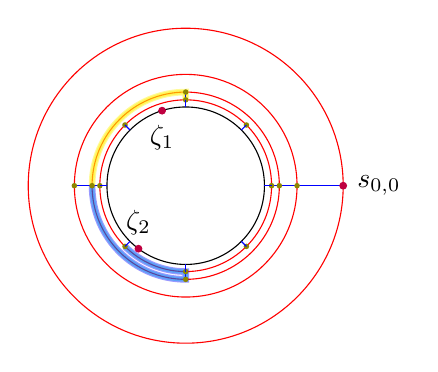
\begin{tikzpicture}
		
		
		\draw (0,0) circle (1);
		\draw[red] (0,0) circle (2);
		\draw[red] (0,0) circle (2^0.5);
		\draw[red] (0,0) circle (2^0.25);
		\draw[red] (0,0) circle (2^0.125);
		
		
		\draw [yellow,-, double=yellow, double distance=4\pgflinewidth, opacity=0.4,
		] (-1.189,0) arc (180:90:1.189) -- (0,1.0905);
		
		\draw [blue,-, double=cyan, double distance=4\pgflinewidth, opacity=0.4,
] (-1.189,0) arc (-180:-90:1.189) -- (0,-1.0905) arc (-90:-135:1.0905);
		
		\draw[blue] (2,0);
		
		\draw[blue] (2,0) --  (1,0);	
		\draw[blue] (-2^0.5,0) -- (-1,0);	
		\draw[blue] (0, 2^0.25) -- (0,1);	
		\draw[blue] (0, -2^0.25) -- (0,-1);	
		
		\fill[olive] (2,0) circle (1pt);
		\fill[olive] (2^0.5,0) circle (1pt);
		\fill[olive] (-2^0.5,0) circle (1pt);
		
		\foreach \angle in {0,90,180,270}
		\fill[olive] (\angle:2^0.25) circle (1pt);
		
		\foreach \angle in {0,45,90,135,180,225,270,315}
		\fill[olive] (\angle:2^0.125) circle (1pt);
		\foreach \angle in {0,45,90,135,180,225,270,315}
		\draw[blue] (\angle:2^0.125) -- (\angle:1);
		
		\node[circle,inner sep=1pt,fill=purple,label=below:{$\zeta_1$}] at (-0.3,0.953) {};

		\node[circle,inner sep=1pt,fill=purple,label=above:{$\zeta_2$}] at (-0.6,-0.8) {};
		
		\node[circle,inner sep=1pt,fill=purple,label={ right:{$s_{0,0}$}} ] at (2,0) {};
	
	\end{tikzpicture}

\caption{A quasiconvexity certificate between two points $\zeta_1,\zeta_2$.} \label{fig:Carleson2}
\end{figure}



\section{Transporting the tracks} \label{rails-section}
For $c \in \heartsuit$, the Julia set of $f_c: z\mapsto z^2+c$ is a Jordan curve. The {\em Böttcher coordinate} $\psi$ is the unique conformal map $\D^{*}\to\Exterior(\mathcal{J}_c)$  which fixes $\infty$ and satisfies the conjugacy relation 
$$
f\circ\psi=\psi\circ f_{0}.
$$
The Böttcher coordinate $\psi$ extends to a homeomorphism between the unit circle $\partial\D$ and $\mathcal{J}_c$ by Carathéodory's
theorem. See \cite[Theorem 9.5]{milnor_book} for a proof of existence, 
relying on the explicit construction 
\begin{equation}
	\psi(z) \, = \, \lim_{n\to \infty} (f_0)^{\circ (-n)} \circ f^{\circ n}\, = \, \lim_{n\to \infty} {(f^{\circ n})}^{1/2^n}.	
\end{equation}

\begin{figure}
    \centering
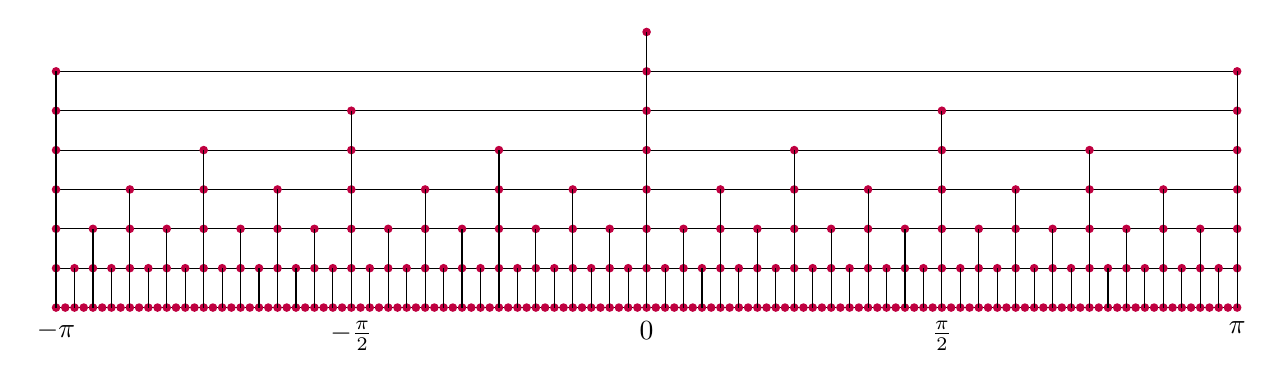
\begin{tikzpicture}[scale=0.5]

  \pgfmathsetmacro{\xlimit}{30}
  \pgfmathsetmacro{\ylimit}{7}

  \foreach \yunscaled in {0,..., \ylimit} 
  {
    \pgfmathsetmacro{\y}{\yunscaled}
    % Draw horizontal lines
    % Draw marked points and vertical lines
    \pgfmathsetmacro{\lognumpoints}{\ylimit-\y}
    \pgfmathsetmacro{\numpoints}{2^\lognumpoints}
    \pgfmathsetmacro{\z}{\xlimit/\numpoints}
    \ifnum\y=\ylimit{
      % Do nothing
    }
    \else{
      \draw (0,\y) -- (\xlimit,\y);
      \foreach \i in {0,...,\numpoints}{
        \pgfmathsetmacro{\x}{\z * \i}
        \draw (\x,\y) node[circle,fill,inner sep=1.1pt, color=purple]{}; % Marked point
      \draw (\x,\y) -- (\x,0); % Vertical line
      }
    }
    \fi
  }
  \draw (\xlimit/2,\ylimit) node[circle,fill,inner sep=1.1pt, color=purple]{}; % Marked point
  \draw (\xlimit/2,\ylimit) -- (\xlimit/2,0); % Vertical line


  % Label horizontal lines
  \draw (0,-0.1) node[below] {$-\pi$};
  \draw (\xlimit/4,-0.1) node[below] {$-\frac \pi 2$};
  \draw (\xlimit/2,-0.1) node[below] {$0$};
  \draw (\xlimit*3/4,-0.1) node[below] {$\frac \pi 2$};
  \draw (\xlimit,-0.1) node[below] {$\pi$};

  % \draw [magenta,-, double=magenta, double distance=4\pgflinewidth, opacity=0.4,
  % ] (0,0.8) -- (1.5,0.8) -- (1.5,0.6) -- (2.25,0.6) -- (2.25,0.4) -- (2.25+0.75/2, 0.4) 
  % -- (2.25+0.75/2, 0.2) -- (2.25+0.75/2+0.75*1/4, 0.2) -- (2.25+0.75/2+0.75*1/4, 0.1);
  % \draw [magenta,-, double=magenta, double distance=4\pgflinewidth, opacity=0.4,
  % ] (6,0.8) -- (6-1.5,0.8) -- (6-1.5,0.6) -- (6-2.25,0.6) -- 
  % (6-2.25,0.4) -- (6-2.25-0.75/2, 0.4) 
  % -- (6-2.25-0.75/2, 0.2) -- (6-2.25-0.75/2-0.75*1/4, 0.2) 
  % -- (6-2.25-0.75/2-0.75*1/4, 0.1)
  % ;
  % \tikzmath{
  %   \curx = 0;
  %   for \step in {1,...,2}{
  %     {\draw [magenta,-, double=magenta, double distance=4\pgflinewidth, opacity=0.4] (\curx, \ylimit-\step) -- (\curx, \ylimit-\step-1);};
  % };}
  % \draw [magenta,-, double=magenta, double distance=4\pgflinewidth, opacity=0.4,
  % ] (0.0, \ylimit-2) -- (\xlimit/4, \ylimit-2) -- (\xlimit/4, \ylimit-3) --
  %  (\xlimit/4+\xlimit/8, \ylimit-3) --
  %  (\xlimit/4+\xlimit/8, \ylimit-4) --
  %  (\xlimit/4+\xlimit/8+\xlimit/16, \ylimit-4) --
  %  (\xlimit/4+\xlimit/8+\xlimit/16, \ylimit-5) --
  %  (\xlimit/4+\xlimit/8+\xlimit/16+\xlimit/32, \ylimit-5) --
  %  (\xlimit/4+\xlimit/8+\xlimit/16+\xlimit/32, \ylimit-6);

  
\end{tikzpicture}
\captionof{figure}{A convenient representation of the dyadic grid in the Böttcher coordinates.
 The horizontal axis is the external angle $\mathrm{Arg}(\psi^{-1}(z))$, and the vertical axis is the equipotential $|\psi ^{-1}(z)|$, plotted on a log scale. 
 The rightmost edge is glued to the leftmost edge.
 Stations are marked in red, and the segments connecting adjacent stations are tracks. An express track is a vertical segment, 
 while a peripheral track is a horizontal segment.
%  The magenta contour bounds the region $\mathcal U_{-1}$.
 }  \label{fig:dyadic_grid}
\end{figure} 


We apply $\psi$ to the tracks that we constructed in $\mathbb D^*$ 
to obtain the corresponding tracks in $\Exterior(\mathcal{J}_c)$:
\begin{definition} \leavevmode
\begin{enumerate}
	\item The 	\emph{stations} of $f_c$ are the points $\psi(s_{n,k})$.


\item The \emph{tracks} of $f_c$ are the curves of the form $\psi (\gamma_{s,s'})$, where $\gamma_{s,s'}$ is a track. They are classified as express or peripheral according to the corresponding classification of $\gamma_{s,s'}$. 
Express tracks lie on the external rays of the filled Julia set $\mathcal K_c$, while peripheral tracks lie on the equipotentials of $\mathcal K_c$.

\item The \emph{itinerary} between a pair of points $(z_1,z_2)$ on $\mathcal J_c$ is
$\eta_{z_1,z_2}=\psi(\eta_{\zeta_1,\zeta_2})$, 
where $\zeta_i=\psi^{-1}(z_i)$ are the corresponding points on $\partial \mathbb D^*$. 
\end{enumerate}

We henceforth omit $c$ and $\psi$ from the notation for ease of reading. It will be clear from the context whether we work in $\mathbb D^*$ or in $\Exterior(\mathcal J)$.

%These itineraries can equivalently be obtained directly as in the case of $\mathbb D^*$, in terms of following the central itineraries from the common ancestor in the tree structure.
%Trivially since $\psi$ is a bijective correspondence between the two decompositions.
\end{definition}

When $c \in (-3/4, 1/4)$, $\psi ((1,\infty))\subseteq\R$ since $\mathcal{J}$ is symmetric with respect to the real line, and in particular, the central station $\psi(s_{0,0})$ lies on the real axis.


\section{Hyperbolic Maps}
In this section we prove the quasiconvexity of $\Exterior(\mathcal J)$ for parameters $c$ in the main cardioid $\heartsuit$. For $c \in \heartsuit$, the dynamics is hyperbolic since the critical point at 0 converges to an attracting fixed point under iteration.

%  Hyperbolic maps enjoy the principle of the conformal elevator, 
%  which roughly says that any ball centered on the Julia set can be blown up to a definite size. 
%  More precisely, we have the following proposition:

% \begin{proposition}[The Principle of the Conformal Elevator] \label{elevator}
% 	Let $f$ be a hyperbolic rational map, $z\in \mathcal J$ be a point on the Julia set of $f$ and $r>0$. There exists some forward iterate $f^{\circ n}$ of $f$ which is injective on the ball $B(z,2r)$ such that
% 	$\diam {f^{\circ n}(B(z,r))}$ is bounded from below uniformly in $z$ and $r$. 
% \end{proposition}


\begin{definition}
	A point $z \in \mathcal J$ is \emph{rectifiably accessible} from $\Exterior(\mathcal J)$ if there is a rectifiable curve $\gamma: [0,1) \to \Exterior(\mathcal J)$ such that $\gamma (t) \to z$ as $t \to 1$.
\end{definition}

% To show quasiconvexity, 
% we need to first show that every point of $\mathcal J$ is rectifiably accessible.
We are now ready to show quasiconvexity in the hyperbolic case:

\begin{theorem}  Let $f:z \mapsto z^2+c$ be a quadratic map with $c \in \heartsuit$. \leavevmode
\begin{enumerate}[label=\normalfont(\roman*)]

\item Given $z\in\mathcal{J}$ decompose its central itinerary into tracks, 
\begin{equation*}
\eta_z = \gamma _1 +\gamma_2 +\dots.
\end{equation*}
We have the estimate
\begin{equation*}
\Length(\gamma_{k})\lesssim\theta^{k},
\end{equation*}
uniformly in $z$, for some constant $\theta=\theta(c)<1$. 
In particular, any point on \(\mathcal{J}\) is rectifiably accessible.

\item The domain $\Exterior(\mathcal{J})$ is quasiconvex with the itineraries $\eta_{z_1,z_2}$ as certificates.
	\end{enumerate}
\end{theorem}

\begin{proof} \leavevmode
(i) For $c=0$, this is a direct computation. 
Suppose $c \neq 0$, and let $\Postcrit$ be the post-critical set of $f$.
Recall that $f: \widehat{\mathbb C} \setminus \Postcrit \to \widehat{\mathbb C} \setminus \Postcrit$
is expanding in the hyperbolic metric by \cref{theorem:hyperbolic_expanding}.

Let $B(0,R) \subset \mathbb{C}$ be a ball large enough that it contains every central itinerary. 
By hyperbolicity, $\Exterior(\mathcal{J}) \cap B(0,R)$ is compactly contained in $\widehat{\mathbb C} \setminus f(\Postcrit)$, and
there is a constant $\theta<1$ such that $\Vert (f^{-1})' \Vert_{\hyp}< \theta$ on $\Exterior(\mathcal{J}) \cap B(0,R)$. Therefore,
\begin{align*}
\HypLength(\gamma_k)  & \leq \theta \cdot \HypLength(f(\gamma_k))\\ & \leq  \dots
	\\ & \leq \theta^k \cdot \HypLength(f^{\circ k}(\gamma_k)),
	\\ & \lesssim \theta^k,
\end{align*}
where the last inequality holds since $f^{\circ k}(\gamma_k)$ lies 
on the real axis in case $\gamma_k$ is an express track, 
or on the equipotential $\psi \bigl (\{ |z| = \sqrt 2\} \bigr )$ otherwise.


As the Euclidean metric is bounded above by a constant multiple of the hyperbolic metric,
we conclude that $\Length(\gamma_k) \lesssim \theta^k$ as well.
Thus any point on $\mathcal J$ can be reached from the central station 
$s_{0,0}$ by a curve of bounded length.

(ii) By (\ref{elevator for points on julia}), 
there exists an $\epsilon>0$ such that any two points are $\epsilon$-apart 
under some iterate of $f$. 
Let $z_{1},z_{2}\in\mathcal{J}(f)$. If $ |z_{1}-z_{2} |\geq\epsilon,$ 
we are done since the length of $\eta_{z_1,z_2}$ is uniformly bounded above by part (i).
On the other hand, if 
$ |z_{1}-z_{2} |<\epsilon$,
then there is an iterate $f^{\circ n}$ for which
\begin{equation}
	|w_1-w_2|:= |f^{\circ n}(z_{1})-f^{\circ n}(z_{2}) |\geq\epsilon,
\end{equation}
so that $\eta_{w_1, w_2}$ is a quasiconvexity certificate.
As $\eta_{w_1, w_2}$ is contained in $\Exterior(\mathcal J) \cap B(0,R)$, it is relatively separated from the post-critical set.
By \cref{koebe-quasiconvexity}, $\eta_{z_1,z_2}$ is also a quasiconvexity certificate.
\end{proof}

 

\section{The Cauliflower}
In this section, $c=\frac 14$ and $f=f_{1/4}: z\mapsto z^2+ \frac 14$.
%The Cauliflower has cusps at the landing points of the dyadic external rays, i.e. the points whose central itinerary has only finitely-many peripheral tracks.
Our goal is to prove the quasiconvexity of $\Exterior(\mathcal{J})$, \cref{quasiconvex-Cauliflower}. 
This is more complicated than the hyperbolic case, 
because the post-critical set $\PostCrit$ of $f$ accumulates at the parabolic fixed point $p=\frac 12$. 
One no longer has a uniform bound on the distortion of inverse iterates, 
and we cannot immediately deduce the quasiconvexity of the itinerary $\eta_{z_1,z_2}$ from the quasiconvexity of $\eta_{w_1,w_2}$ using Koebe's distortion theorem. 
As a substitute, we present an analogue of the principle of the conformal elevator in this parabolic setting.

\subsection{Itineraries have finite length}
\label{sec:finite-length}

We first show that each itinerary $\eta_{z_1,z_2}$ has a finite length. 
We will in fact show an exponential decay of the lengths of the constituent tracks. 
For this to hold it is necessary to glue together consecutive express tracks: 
for example, the tracks in the central itinerary that lies on the real axis, $\eta_{1/2}$, 
have only a quadratic rate of length decay. To fix this, we introduce:

\begin{definition}
	The \emph{reduced decomposition} of an itinerary $\eta$ is the unique decomposition $\eta=\gamma_1 + \delta_1 + \dots$ where each $\gamma_i$ is a concatenation of express tracks and $\delta_i$ consists of a single peripheral track.
\end{definition}

\begin{proposition} \label{prop:finite-length}
	Let $z \in \mathcal J$, and let $\eta_z= \gamma_1 + \delta_1 + \dots  $ be the reduced decomposition of its central itinerary. Then $\Length(\gamma_k)\lesssim \theta^k$ and $\Length(\delta_k)\lesssim \theta^k$ for some $\theta < 1$. Thus $\Length(\eta_z)$ is finite and uniformly bounded over $z \in \mathcal J$, and all points $z\mathcal \in \mathcal J$ are rectifiably accessible.
\end{proposition}

% !TEX root = main.tex

\begin{figure}
    \centering
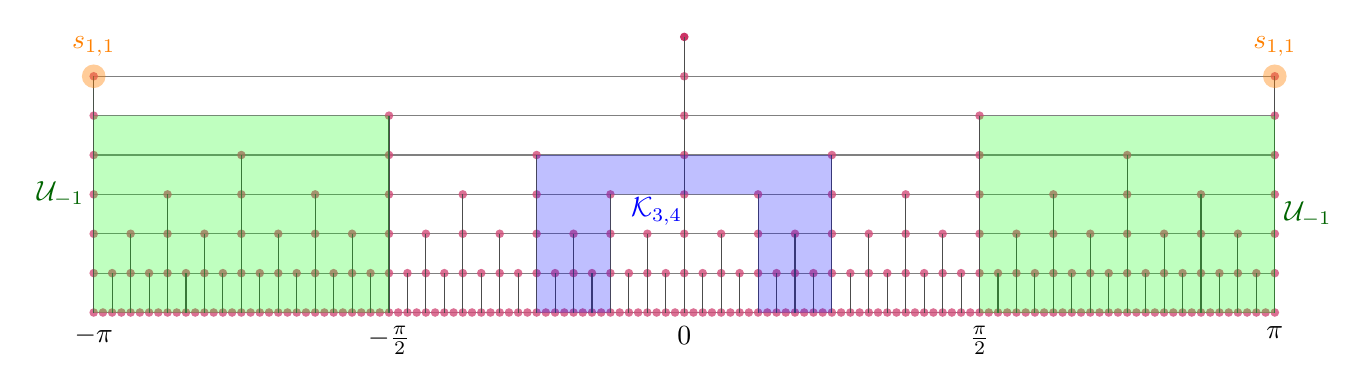
\begin{tikzpicture}[scale=0.5]

\pgfmathsetmacro{\xlimit}{30}
\pgfmathsetmacro{\ylimit}{7}

  \foreach \yunscaled in {0,..., \ylimit} 
  {
    \pgfmathsetmacro{\y}{\yunscaled}
    \pgfmathsetmacro{\lognumpoints}{\ylimit-\y}
    \pgfmathsetmacro{\numpoints}{2^\lognumpoints}
    \pgfmathsetmacro{\z}{\xlimit/\numpoints}
    \ifnum\y=\ylimit{
      % Do nothing!
    }
    \else{
      \draw  [color=black!50!white] (0,\y) -- (\xlimit,\y);
      \foreach \i in {0,...,\numpoints}{
        \pgfmathsetmacro{\x}{\z * \i}
        \draw (\x,\y) node[circle,fill,inner sep=1.1pt, color=purple!70!white, opacity=0.8]{}; % Marked point
      \draw [color=black!70!white]  (\x,\y) -- (\x,0); % Vertical line
      }
    }
    \fi
  }
  \draw (\xlimit/2,\ylimit) node[circle,fill,inner sep=1.1pt, color=purple,opacity=0.8]{}; % Marked point
  \draw [color=black!70!white] (\xlimit/2,\ylimit) -- (\xlimit/2,0); % Vertical line


  % Label horizontal lines
  \draw (0,-0.1) node[below] {$-\pi$};
  \draw (\xlimit/4,-0.1) node[below] {$-\frac \pi 2$};
  \draw (\xlimit/2,-0.1) node[below] {$0$};
  \draw (\xlimit*3/4,-0.1) node[below] {$\frac \pi 2$};
  \draw (\xlimit,-0.1) node[below] {$\pi$};



\definecolor{darkgreen}{RGB}{0,100,0}
\fill [green, opacity=0.25] 
  (0,\ylimit-1)
  --(0,\ylimit-2) 
  -- (\xlimit/4,\ylimit-2)
   -- (\xlimit/4,\ylimit-7)
  -- (0,\ylimit-7)
  --cycle
  node[midway, left, opacity=1,text=darkgreen] {$\mathcal U_{-1}$};;  

    \fill [blue, opacity=0.25] 
(\xlimit/4+\xlimit/8, \ylimit-3)
-- (\xlimit/4+\xlimit/8, 0)
-- (\xlimit/4+\xlimit/8+\xlimit/16, 0)
-- (\xlimit/4+\xlimit/8+\xlimit/16, \ylimit-4)
-- (\xlimit/4+\xlimit/4+\xlimit/16, \ylimit-4)
-- (\xlimit/4+\xlimit/4+\xlimit/16, 0)
-- (\xlimit/4+\xlimit/4+\xlimit/8, 0)
-- (\xlimit/4+\xlimit/4+\xlimit/8, \ylimit-3)
--cycle
       node[midway, below, yshift=-12,opacity=1, xshift=-10] {$\mathcal K_{3,4}$};
; 

\fill[orange, opacity=0.4] (\xlimit, 6) circle (0.3) node[label={[opacity=1]:$s_{1,1}$}]{};

\fill[orange, opacity=0.4] (0, 6) circle (0.3) node[label={[opacity=1]:$s_{1,1}$}]{};


\fill [green, opacity=0.25] 
        (\xlimit-0,\ylimit-2)
    -- (\xlimit-\xlimit/4,\ylimit-2)
    --(\xlimit-\xlimit/4, \ylimit-7)
    --(\xlimit, \ylimit-7)
    -- cycle
       node[midway, right, opacity=1, text=darkgreen] {$\mathcal U_{-1}$};
;

\end{tikzpicture}
\captionof{figure}{
Using the dyadic representation from \cref{fig:dyadic_grid},
 the domain $\mathcal U_{-1}$ is highlighted in green, and the domain $\mathcal K_{3,4}$ is highlighted in purple.
 The station $s_{1,1}$ is highlighted in orange; recall that points with external angle $\pm \pi$ appear twice in this representation. 
 %Also notice that every itinerary passing through the station $s_{1,1}$ must continue vertically from it.
 }  \label{fig:dyadic_grid_regions}
\end{figure} 


For the proof, let $\mathcal U_{-1}$ be the Jordan domain enclosed by the Julia set $\mathcal J$, 
the rightmost itinerary starting from the pre-central station and the leftmost one. 
See \cref{fig:dyadic_grid_regions}.
This domain is constructed so that it contains all itineraries that start at the station 
$s_{1,1} = \psi(-\sqrt{2})$, the preimage of the central station under $f$. 
Notice that $\mathcal U_{-1}$ is compactly contained in $\widehat{\mathbb C} \setminus \Postcrit$, because the post-critical set $\PostCrit \subset [0,1/2] \cup \{\infty\}$ touches the Julia set $\mathcal J$ only at $p=1/2$, which is not contained in $\overline{\mathcal U_{-1}}$.

The crucial property of the domain $\mathcal U_{-1}$ is: 
% call $s_{-1}:=s_{1,1}$ the \emph{pre-central station}

\begin{lemma} \label{lemma-enough-visits-of-premain_station}
	Let $\gamma = \gamma_1 + \delta_1 + \dots $ be the reduced decomposition of an itinerary $\gamma$. Then for every $k > 1$, there exist $k-1$ iterates $n_1 < \dots < n_{k-1}$ such that $f^{\circ {n_i}}(\gamma_k) \subset \mathcal U_{-1}$. % This is actually an off-by-1 lie, since n_1=0 has no predecessor.
\end{lemma}

\begin{proof}
	Every station $s \not \in (0, \infty)$ has a first iterate $f^{\circ n_s}(s)$ lying on the negative real axis $(-\infty, 0)$.
	For any $i \in \{2, \dots, k-1\}$, let $s_i$ be the first station of $\gamma _i$ and take $n_i := n_{s_i}$. % Note s_i is not on the positive axis since $i \geq 2$. 
	By the definition of $\,\mathcal U_{-1}$, the itinerary $f^{\circ n_i}(\gamma)$ is contained in  $\,\mathcal U_{-1}$ from the station $f^{\circ n_i}(s_i)$ onwards, and in particular $f^{\circ n_i}(\gamma_k) \subset \mathcal U_{-1}$.
\end{proof}
\begin{proof}[Proof (\cref{prop:finite-length})] 
By \cref{theorem:hyperbolic_expanding}, there is a uniform bound $\Vert (f^{-1})' \Vert_{\hyp}< \theta < 1$ on $\mathcal U_{-1}$
with respect to the hyperbolic metric of the domain $\widehat{\mathbb C} \setminus \Postcrit$, for both branches of $f^{-1}$ defined in $\mathcal U_{-1}$. 

In the notation of \cref{lemma-enough-visits-of-premain_station}, we then have 
\begin{align*}
	\HypLength(\gamma_k)  &  \leq \HypLength(f^{\circ (n_1-1)}(\gamma_k)) \\ 
	& \leq \theta \cdot \HypLength(f^{\circ n_1}(\gamma_k))\\
	& \leq  \dots \\
	 & \leq \theta^k \cdot \HypLength(f^{\circ n_k}(\gamma_k)) \\
	 & \lesssim \theta^k.
\end{align*}
As the Euclidean metric is bounded above by a constant multiple of the hyperbolic metric, we infer that $\Length(\gamma_k) \lesssim \theta^k$.
\end{proof}


\subsection{Some Estimates and Notation}

To estimate the length of express tracks, we introduce the notations $s_n := s_{n, 0}$ and 
\begin{equation}
	\ell_n := \Length([s_{n},s_{n+1}]) = s_{n}-s_{n+1}.
\end{equation}
From the definition of the stations $s_n$, we have $f(s_{n+1}) = s_n$ for all $n \ge 0$. Since the Cauliflower is symmetric with respect to the real line, the $s_n$ are positive real numbers converging to the cusp at $p = \frac{1}{2}$.

\begin{lemma} \label{lem-ell_n}
	The lengths ${\ell_n}$ satisfy:
	
	{\em (i)}
	\begin{equation}
	\label{eq:ell_n1}
		\frac {|p-s_n|}{\ell_n} \to \infty,
	\end{equation}
	
	{\em (ii)}
	\begin{equation}
	\label{eq:ell_n2}
		\frac{\ell_n}{\ell_{n+1}} \to 1.
	\end{equation}
	In particular, for any $C > 0$, there is a sufficiently large integer $d$ such that
	\begin{align*}
		\ell_{m}+\ldots+\ell_{n} \geq C (\ell_m+\ell_n)
	\end{align*}
	whenever $|m-n| \geq d$.
\end{lemma}

\begin{proof}[Sketch of proof] Recall that $s_n$ satisfy the recurrence
\begin{equation}
s_{n+1}^2 + 1/4 =f(s_{n+1})= s_n.
\end{equation}
Consequently, 
the sequence of positive numbers
$$
a_n = s_n-\frac{1}{2}
$$
satisfies the recurrence 
\begin{equation}
a_n = a_{n+1}^2+a_{n+1}.
\end{equation}

An induction argument shows that $a_n = 1/n + o(1/n)$, and consequently, $\ell_n = a_n - a_{n+1} \asymp 1/n^2$.
% Notice that it is not true in general that if a_n \asymp 1/n then a_n-a_{n-1} \asymp 1/n^2.

% % The full proof by induction:
% % It is enough to prove that for every $\epsilon>0$ there exists $k = k(\epsilon)$
% % for which $a_n \overset{\epsilon}{\asymp}  \frac 1{n+k}$,
% % meaning that for all large enough $n$,
% % we have 
% % \[e^{-\epsilon} \leq \left | \frac {a_n}{1/(n+k)} \right |\leq e^\epsilon.\]
% % This is enough because then since $\frac 1n \overset{\epsilon}{\asymp} \frac 1{n+k}$ we deduce 
% % $$
% % a_n \overset{2\epsilon}{\asymp} \frac 1n.
% % $$
% % % Can this technicality be avoided?
% % Let $\epsilon >0$, and assume that 
% % $$\frac 1n \leq a_k \leq \frac {1+\epsilon}n.$$
% % We deduce from it that
% % $$\frac 1{n+1} \leq a_{k+1} \leq \frac {1+\epsilon}{n+1}.$$
% % Notice that such an element $a_k$ exists in some range of the form $[\frac 1n, \frac {1+\epsilon}n]$ because $a_n \to 0$. 
% % For the induction step, we have two parts:

% % For the first inequality, assume by contradiction that $a_{k+1}<\frac 1{n+1}$. Then 
% % $$\frac 1n \leq a_k < \frac 1{n+1} + \frac 1{(n+1)^2}$$
% % which is a contradiction.

% % For the second inequality, assume by contradiction that 
% % $$a_{k+1}> \frac {1+\epsilon}{n+1}.$$
% % Then 
% % $$
% % \frac {1+\epsilon}n \geq a_k > \frac {1+\epsilon}{n+1}
% % + \frac {(1+\epsilon)^2}{(n+1)^2},
% % $$
% % which is equivalent to
% % $\frac {1}{n} >
% % \epsilon.$ 
% % This is again a contradiction, and we are done.

\end{proof}

% If an itinerary $\gamma$ is relatively separated from $\PostCrit$, then the preimages of $\gamma$ under $f$ have bounded distortion. 
% In particular, if $\gamma$ is a quasiconvexity certificate, 
% then Koebe's distortion theorem implies that $f^{-1}(\gamma)$ is also a certificate with a comparable constant.


\begin{lemma}
\label{expansion factor}
There exists a constant $k>0$ such that for any pair of points $z_1, z_2 \in \mathcal J$, we have 
$|f(z_1)-f(z_2)| \leq k|z_1-z_2|$.
\end{lemma}

\begin{proof}
	We have 
	\begin{equation}
		|f(z_1)-f(z_2)| \, = \,  \biggl | \int_{z_1} ^{z_2} f'(z) dz \biggr | 
  \, \leq \, k|z_1-z_2|	
	\end{equation}
for $k=\max_{z \in B} |f'(z)|$, where $B$ is any ball containing $\mathcal J$. 
\end{proof}
 
\subsection{Dynamics near the parabolic fixed point}

The purpose of the following definition is to organize points on the Julia set $\mathcal J$ according to their distance from the main cusp $p=1/2$ in an $f$-invariant way. We decompose the points of $\mathcal J$ according to the first \emph{departure}\,: the first station at which the central itinerary makes a turn.

\begin{figure}
    \centering
    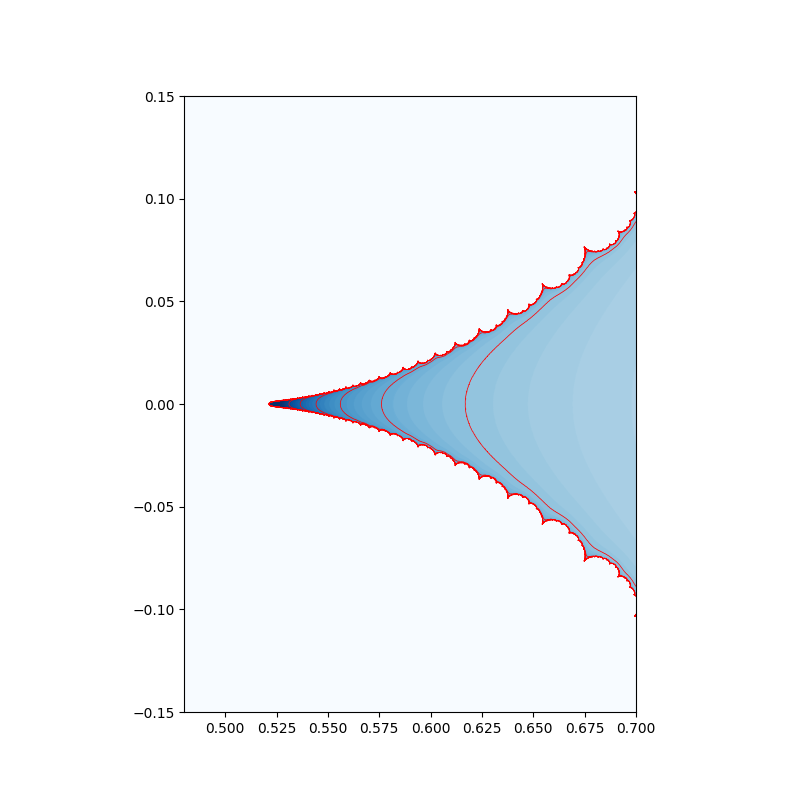
\includegraphics[width=\textwidth]{figures/cauliflower_equipotentials2.png}
    \caption{The Cauliflower near the parabolic point $p=1/2$.}
    \label{fig:my_figure}
\end{figure}
\begin{figure}
	\centering
	
	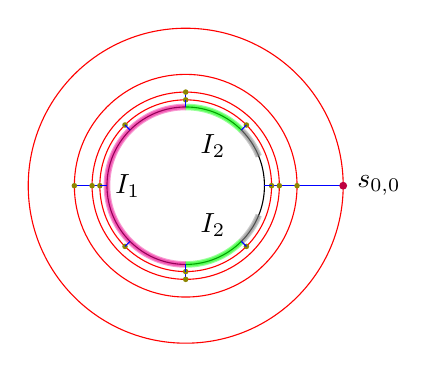
\begin{tikzpicture}
		
		
		\draw (0,0) circle (1);
		\draw[red] (0,0) circle (2);
		\draw[red] (0,0) circle (2^0.5);
		\draw[red] (0,0) circle (2^0.25);
		\draw[red] (0,0) circle (2^0.125);
		
		
		\draw [magenta,-,
			double=magenta,
			double distance=4\pgflinewidth, opacity=0.4,
			] (0,1) arc (90:270:1);
		
		\draw [green,-,
			double=green,
			double distance=4\pgflinewidth, opacity=0.4,
			] (0,1) arc (90:45:1);

		\draw [green,-,
			double=green,
			double distance=4\pgflinewidth, opacity=0.4,
			] (0,-1) arc (270:315:1);

		\draw [gray,-,
			double=gray,
			double distance=4\pgflinewidth, opacity=0.4,
			] (45:1) arc (45:22:1);
		\draw [gray,-,
			double=gray,
			double distance=4\pgflinewidth, opacity=0.4,
			] (-45:1) arc (-45:-22:1);

		
		\draw[blue] (2,0);
		
		\draw[blue] (2,0) --  (1,0);	
		\draw[blue] (-2^0.5,0) -- (-1,0);	
		\draw[blue] (0, 2^0.25) -- (0,1);	
		\draw[blue] (0, -2^0.25) -- (0,-1);	
		
		\fill[olive] (2,0) circle (1pt);
		\fill[olive] (2^0.5,0) circle (1pt);
		\fill[olive] (-2^0.5,0) circle (1pt);
		
		\foreach \angle in {0,90,180,270}
		\fill[olive] (\angle:2^0.25) circle (1pt);
		
		\foreach \angle in {0,45,90,135,180,225,270,315}
		\fill[olive] (\angle:2^0.125) circle (1pt);
		\foreach \angle in {0,45,90,135,180,225,270,315} 		
		\draw[blue] (\angle:2^0.125) -- (\angle:1);
		
		
		\node[circle,inner sep=1pt,label=left:{$I_1$}] at (-0.4,0) {};

		\node[circle,inner sep=1pt,label=right:{$I_2$}] at (0.01,0.5) {};
		\node[circle,inner sep=1pt,label=right:{$I_2$}] at (0.01,-0.5) {};
		
		\node[circle,inner sep=1pt,fill=purple,label=right:{$s_{0,0}$}] at (2,0) {};
		
	\end{tikzpicture}
	
	\caption{First few parts of the departure decomposition $I_m$ of the circle.
	} \label{fig:departure-decomposition}
\end{figure}


\begin{definition}

Let $n \in \mathbb N$. We define the $n$-th \emph{departure set} $I_{n, \mathbb D} \subset \partial \mathbb D ^*$ to be the set of points $\zeta \in \partial \mathbb D^*$ whose central itinerary $\eta_{\zeta}$ starts with $n$ express tracks, followed by a peripheral track.
See \cref{fig:departure-decomposition}.
\end{definition}

This decomposition is invariant under $f_0$ in the sense that $f_0(I_{n+1, \mathbb D})=I_{n, \mathbb D}$, because of the invariance of $\eta _\zeta$.
Applying the Böttcher map $\psi$, we obtain a corresponding departure decomposition $I_n = \psi(I_{n, \mathbb D})$ of $\mathcal J$ that is invariant under $f$.

We now use this decomposition to analyze the case where the points $w_1,w_2$ lie in ``well-separated cusps''. Namely, suppose that
\begin{align} \label{parabolic separation}
	w_1 \in I_n, \quad w_2 \in I_m, \quad m-n > d,
\end{align}
where $d$ is a sufficiently large integer, to be chosen later. 
This will give some control from below on $|w_1-w_2|$. 
We represent the itinerary $\eta=\eta_{w_1,w_2}$ as a concatenation of three paths: the radial segment $\gamma_{m,n}=[s_{m,0},s_{n,0}]$ and the two other components, $\gamma _m$ and $\gamma_n$. See \cref{fig:Three-parts-of-eta} for the picture in the exterior unit disk.
Thus we have
\begin{equation}
\begin{split}    
\Length(\eta) &=\Length(\gamma_m)+\Length(\gamma_{m,n})+\Length(\gamma_n) \\ 
&= \Length(\gamma_m)+\ell_m + \dots +\ell_{n-1}+\Length(\gamma_n).
\end{split}
\end{equation}

\begin{figure}
	\centering
	
	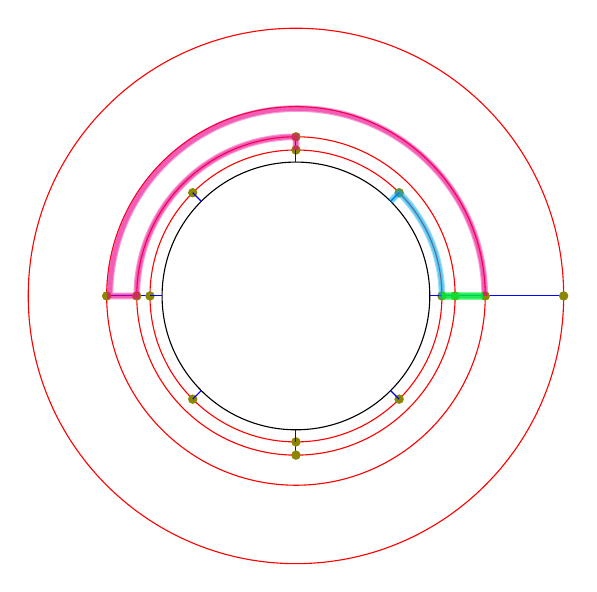
\begin{tikzpicture}[scale=1.7]
		
		
		\draw (0,0) circle (1);
		\draw[red] (0,0) circle (2);
		\draw[red] (0,0) circle (2^0.5);
		\draw[red] (0,0) circle (2^0.25);
		\draw[red] (0,0) circle (2^0.125);
		
		
		\draw[blue] (2,0);
		
		\draw[blue] (2,0) --  (1,0);	
		\draw[blue] (-2^0.5,0) -- (-1,0);	
		\draw[blue] (0, 2^0.25) -- (0,1);	
		\draw[blue] (0, -2^0.25) -- (0,-1);	
		
		\fill[olive] (2,0) circle (1pt);
		\fill[olive] (2^0.5,0) circle (1pt);
		\fill[olive] (-2^0.5,0) circle (1pt);
		
		\foreach \angle in {0,90,180,270}
		\fill[olive] (\angle:2^0.25) circle (1pt);
		
		\foreach \angle in {0,45,90,135,180,225,270,315}
		\fill[olive] (\angle:2^0.125) circle (1pt);
		\foreach \angle in {0,45,90,135,180,225,270,315} 		
		\draw[blue] (\angle:2^0.125) -- (\angle:1);
		
		

\draw [magenta,-,
double=magenta,
double distance=4\pgflinewidth, opacity=0.4,
] (1.41,0) arc (0:180:1.4) -- (-1.189,0) arc (180:90:1.189) -- (0,1.0905);

\draw [cyan,-,
double=cyan,
double distance=4\pgflinewidth, opacity=0.4,
] (1.4,0) -- (1.0905,0) arc (0:45:1.0905) -- (45:1) ;


\draw [green,-,
double=green,
double distance=6\pgflinewidth, opacity=0.4,
] (1.0905,0) -- (1.4,0);


\draw[blue] (2,0);

		
	\end{tikzpicture}
	
	\caption{The three parts of an itinerary $\eta$. The green path is  $\gamma _{m,n}$,  the cyan and magenta are $\gamma _m$ and $\gamma_n$.
	} \label{fig:Three-parts-of-eta}
\end{figure}



The condition $m-n \geq d$ prevents the line segment $\gamma _{m,n}$ from being small in comparison to $\gamma_m$ and $\gamma_n$:
\begin{proposition}
\label {case-3-proof}
There exists a sufficiently large integer $d$ so that for every pair of points $w_1,w_2 \in \mathcal J$ satisfying $w_1\in I_m$ and $w_2 \in I_n$ with $m-n \geq d$, we have
	\begin{equation}
	\label{eq:triangle-comparison}
		\Length(\gamma_{m,n}) \asymp |w_1-w_2|.
	\end{equation}
Moreover, the itinerary $\eta_{w_1,w_2}$ is a quasiconvexity certificate.
\end{proposition}

We henceforth fix a value of $d$ as in the proposition.
\begin{proof} 
We first make two elementary observations. Since both the paths $\gamma_m$ and the segments $[s_{n,0},s_{n+1}]$ of length $\ell_n$ are equivariant under $f$, Koebe's distortion theorem applied to the iterates of $f^{-1}$ shows that $\Length(\gamma_m) \asymp \ell_m$. In particular,
\begin{equation} \label{eq:gamma_m_not_large}
		\Length(\gamma_m) \leq C \ell_m,
	\end{equation}
for some constant $C \geq 0$.  \textcolor{red}{Maybe there is no branch of $f^{\circ -(m-n)}$ defined in a neighborhood of both $\gamma_m$ and $\ell_m$?} Notice that (\ref{eq:gamma_m_not_large}) holds for $m=1$ by \cref{prop:finite-length}, which gives a uniform bound on the length of an itinerary.

Meanwhile, by \cref{lem-ell_n}, there exists an integer $d$ such that
\begin{align}
C(\ell_m + \ell _n) \leq \frac{\Length(\gamma_{m,n})}{2}
\end{align}
whenever $m-n \geq d$.

By the triangle inequality, we have
\begin{align*} 
		\bigl | \Length(\gamma_{m,n}) - |w_1-w_2| \bigr | & \le \Length(\gamma_m)+\Length(\gamma_n) \\
		& \le \frac{\Length(\gamma_{m,n})}{2},
\end{align*}
which clearly implies (\ref{eq:triangle-comparison}) and thereby that $\eta_{w_1,w_2}$ is a certificate.
\end{proof}

\bigskip

\begin{figure}
    \centering
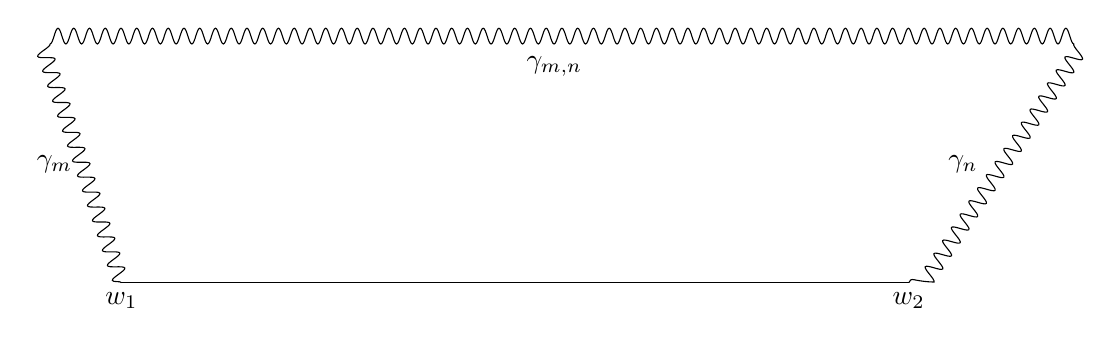
\begin{tikzpicture}
	% draw the points w1 and w2
	\coordinate[label=below:$w_1$] (w1) at (0,0);
	\coordinate[label=below:$w_2$] (w2) at (10,0);
        \coordinate[] (s1) at (-1,3);
        \coordinate[] (s2) at (12,3);

 
	% draw a straight line between w1 and w2
	\draw (w1) -- (w2);
	
	% draw a wiggly path from w1 to w2
	\draw [decorate,decoration={snake,segment length=2mm,amplitude=1mm}, label=below:$\gamma_m$] (w1) -- node[left] {$\gamma_m$} (s1) -- node[below] {$\gamma_{m,n}$} (s2) -- node[left] {$\gamma_n$} (w2);
\end{tikzpicture}
\captionof{figure}{
 Schematic illustration of the proof of \cref{case-3-proof}.
 }  \label{fig:proof-triangle-ineq}
\end{figure}


\subsection{Quasiconvexity: three special cases}

We now show that the itineraries $\eta_{w_1,w_2}$ are certificates in three special cases. To state them, we introduce some notation.

\subsubsection{Notation}

For each $n$, we denote by  $\alpha_n$ the union of the two outermost tracks emanating from the station $s_{n,0}$. 
Notice that the curves $\alpha_n$ are pairwise disjoint since this is true for their pullbacks to the exterior unit disk.

We define the constants $C_1, C_2, \epsilon$ as follows. We first choose $C_1 \ge 2$, then we let $C_2 = C_1 + d+2$ and choose $\epsilon >0$ small enough so that we have 
\begin{equation}
	\dist(\alpha_{C_2}, \alpha_{C_1}) \geq k \cdot \epsilon,
\end{equation}
where the constant $k$ was defined in \cref{expansion factor}.
The constant $C_2$ was chosen so that for any pair $(m,n)$ of integers, we have at least one of the following three cases: either $m,n$ are both greater than $C_1$, or both are smaller than $C_2$, or $|m-n| > d$.

\subsubsection{Three Special Cases}
In this section we treat the following special cases:
\begin{enumerate}
	\item $|w_1-w_2| \geq  \epsilon$, $\quad |m-n|<d$, $\quad 2 \le m,n < C_2$; %relatively separated
	\item $|w_1-w_2| \geq \epsilon$, $\quad |m-n|<d$, $\quad  m,n> C_1$; %relatively separated
	\item $|w_1-w_2| \leq k \epsilon$, $\quad |m-n| \geq d$.
\end{enumerate}

Notice that Case 2 overlaps with Case 1.
 We denote the domain enclosed by $\alpha_m, \alpha_n$ and $\mathcal J$ by $\mathcal K_{m,n}$, and denote the domain enclosed by $\mathcal J$ and $\alpha_n$ by $\mathcal K_n$.

\begin{lemma}
Let $w_1 \in I_m$ and $w_2 \in I_n$, for $n \geq m \geq 2$. Then the itinerary $\eta_{w_1,w_2}$ is contained in the domain $\mathcal K_{m,n+1}$.
\end{lemma}

\begin{proof}
    This follows from the combinatorics of the construction in the exterior unit disk. 
\end{proof}

\begin{lemma}
\label{case 1 rel. sep}
Let $w_1,w_2 \in \mathcal J$. In Cases 1 and 2, $\eta_{w_1,w_2}$ is relatively separated from the post-critical set. In each of the three special cases, the itinerary $\eta_{w_1,w_2}$ is a quasiconvexity certificate. 
\end{lemma}

\begin{proof}
\emph{Case 1.} In this case, the itinerary is contained in the domain $\mathcal K_{2, C_2+1}$.
Since $\dist(\mathcal K_{2, C_2+1}, \mathcal P)>0$, $\eta_{w_1,w_2}$ is $\eta$-relatively separated for some $\eta>0$. 

\emph{Case 2.}
Assuming without loss of generality that $n \geq m$, the itinerary is contained in $\mathcal K_{m,n+1}$. By Koebe's distortion theorem, $\eta_{w_1,w_2}$ is also relatively separated.
{\large \textcolor{red}{Why?}}

Thus the itineraries in Case 1 and in Case2 are certificates, by \cref{koebe-quasiconvexity}.

\emph{Case 3} is the content of \cref{case-3-proof}.
\end{proof}

\subsection{Quasiconvexity: general case}
We apply a stopping time argument to promote the quasiconvexity of $\eta_{w_1,w_2}$ to the quasiconvexity of $\eta_{z_1,z_2}$, thereby proving the following theorem:

\begin{theorem} \label{quasiconvex-Cauliflower}
	The domain $\Exterior(\mathcal{J})$ is quasiconvex, with the itineraries $\eta_{z_1,z_2}$ as certificates.
\end{theorem}

\begin{proof}[Proof. (Parabolic Conformal Elevator on $\mathcal J$)] \label{parabolic-elevator}
Let  $(z_1,z_2)$ be a pair of points on $\mathcal J$. 
If $|z_{1}-z_{2}| \geq \epsilon,$ 
we are done since the length of $\eta_{z_1,z_2}$ is uniformly bounded above by  \cref{prop:finite-length}.

It remains to treat the case when $|z_{1}-z_{2}| \le \epsilon$. By  \cref{parabolic elevator for points on julia} and \cref{expansion factor}, we may repeatedly apply $f$ to $(z_1, z_2)$ until either of the three special cases occurs.
Denote by $w_i=f^{\circ N}(z_i)$ the resulting points. We have already proved that the itinerary $\eta_{w_1,w_2}$ satisfies
\begin{equation*}
	\Length(\eta_{w_1,w_2}) \leq A |w_1-w_2|,
\end{equation*}
for some $A>0$. We now show that the original pair of points $(z_1,z_2)$ enjoys a similar estimate,
\begin{equation*}
	\Length(\eta_{z_1,z_2}) \leq C |z_1-z_2|,
\end{equation*}
where $C$ depends only on $A$.

In Cases 1 and 2, we are done by \cref{case 1 rel. sep}. In Case 3, 
the itinerary $\eta_{w_1,w_2}$ is contained in $\mathcal K_2$. Let $\mathcal K_{-2}$ be the preimage of $\mathcal K_2$ under $f$ that contains the negative preimage $f^{-1}(p)=-\tfrac 12$ of the cusp $p$. 
As the domain $\mathcal K_{-2}$ is relatively separated from $\PostCrit$ and contains the curve 
$f^{\circ (N-1)}(\eta_{z_1,z_2}) = \eta_{f^{-1}(w_1),f^{-1}(w_2)}$,
we may use Koebe's distortion theorem and \cref{koebe-quasiconvexity} to conclude that
\begin{equation}
	\frac{\Length(\eta_{z_1,z_2})}{|z_1-z_2|} \, \asymp \,
		\frac{\Length(\eta_{f^{-1}(w_1),f^{-1}(w_2)})}{|f^{-1}(w_1)-f^{-1}(w_2)|} \, \asymp \,
		\frac{\Length(\eta_{w_1,w_2})}{|w_1-w_2|}
\end{equation}
as desired.
\end{proof}

% \bibliographystyle{acm}
\bibliographystyle{ACM-Reference-Format}
\bibliography{main}

 
\nomenclature{$k$}{The constant guaranteed by 
\cref{expansion factor}.}
% \nomenclature{$\mathbb{D}^*$}{The exterior of the unit disk, $\{|z| >1 \}$.}
\nomenclature{$\mathbb{D}^*$}{The exterior of the unit disk.}
\nomenclature{$d$}{An integer for which itineraries connecting $w_1\in I_m$ with $w_2\in I_n$ for $m-n \geq d$ are certificates. Defined in \cref{case-3-proof}.}
\nomenclature{$f, f_c$}{The map $z \mapsto z^2+c.$}
\nomenclature{$\mathcal J$}{The Julia set of $f$.}
\nomenclature{$\mathcal K$}{The filled Julia set of $f$.}
\nomenclature{$\gamma_{z_1, z_2}$}{The track connecting $z_1$ and $z_2$. It can be either angular (\enquote{peripheral}) or radial (\enquote{express}).}
\nomenclature{$\eta_{z_1, z_2}$}{The itinerary connecting two points. When $z_1$ and $z_2$ are stations, this is the same as $\gamma_{z_1,z_2}$.}
\nomenclature{$A_\infty(f)$}{The exterior of the Julia set of $f$. The complement of $\mathcal K$.}
\nomenclature{$\mathrm{Exterior}(\mathcal{J})$}{ $\;$ An alternative notation for $A_\infty(f_c)$.}
\nomenclature{$\psi$}{The Böttcher coordinate $\mathbb D ^* \to \Exterior(\mathcal J)$ conjugating $f_0$ and $f$.}
\nomenclature{$s_{n,k}$}{A station in $\mathbb D^*$ or its image under $\psi$.}
\nomenclature{$\Delta (\gamma, \mathcal P)$}{The relative distance to the post-critical set.}
\nomenclature{$I_{n}$}{The $n$-th departure set.}
\nomenclature{$\ell_n$ }{$\Length([s_{n},s_{n+1}]) = s_{n,0}-s_{n+1,0}.$}
\nomenclature{$\alpha_n$}{The union of the two outermost tracks emanating from the station $s_{n,0}$.}

\printnomenclature
\end{document}
